\chapter{States with more than one infrared phonons}

Section about the states with 2 and 3 infrared phonons and their particular behaviour.

\section{Energy renormalization}

At large $\lambda_{ir}$ we recover the harmonic behaviour. This is analog to have a spring with a displaced equilibrium position.

\section{Projection into phonon coordinates}

State with two infrared phonons:

\begin{figure}[ht!]
\centering
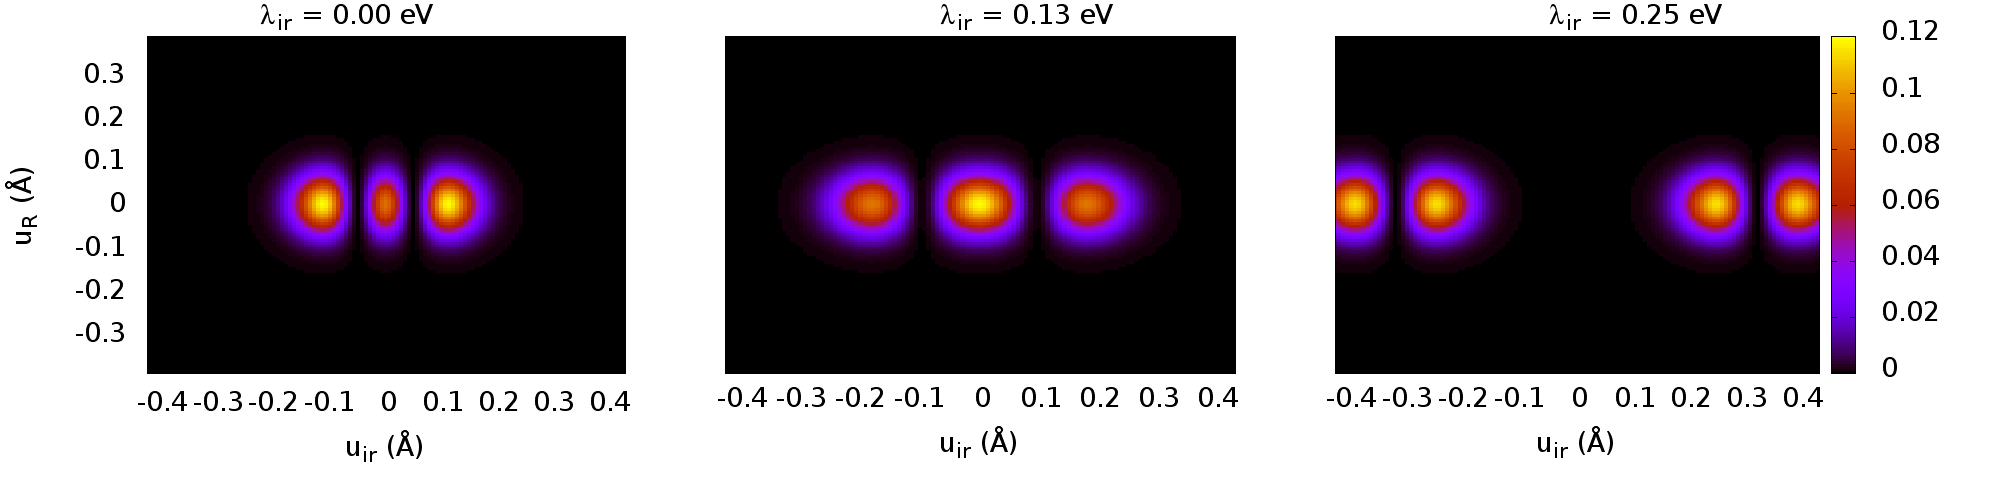
\includegraphics[width=0.8\textwidth]{images/ph-second_infrared.png}
\caption{Projection into phonon coordinates of the state with 2 infrared phonons.}
\label{fig:ph-second_infrared}
\end{figure}

State with three infrared phonons:

\begin{figure}[ht!]
\centering
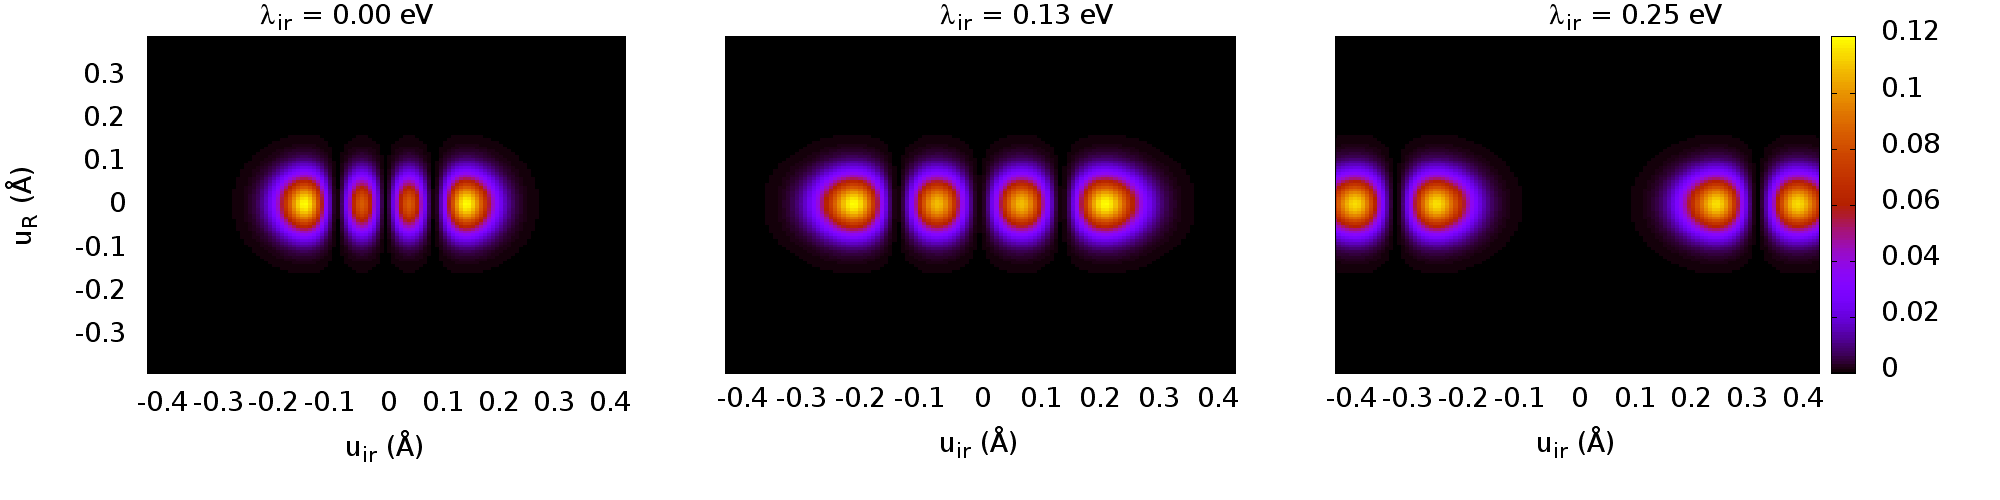
\includegraphics[width=0.8\textwidth]{images/ph-third_infrared.png}
\caption{Projection into phonon coordinates of the state with 3 infrared phonons.}
\label{fig:ph-third_infrared}
\end{figure}

\section{Isotopic shifts}

The isotopic shifts are different:

\begin{figure}[ht!]
\centering
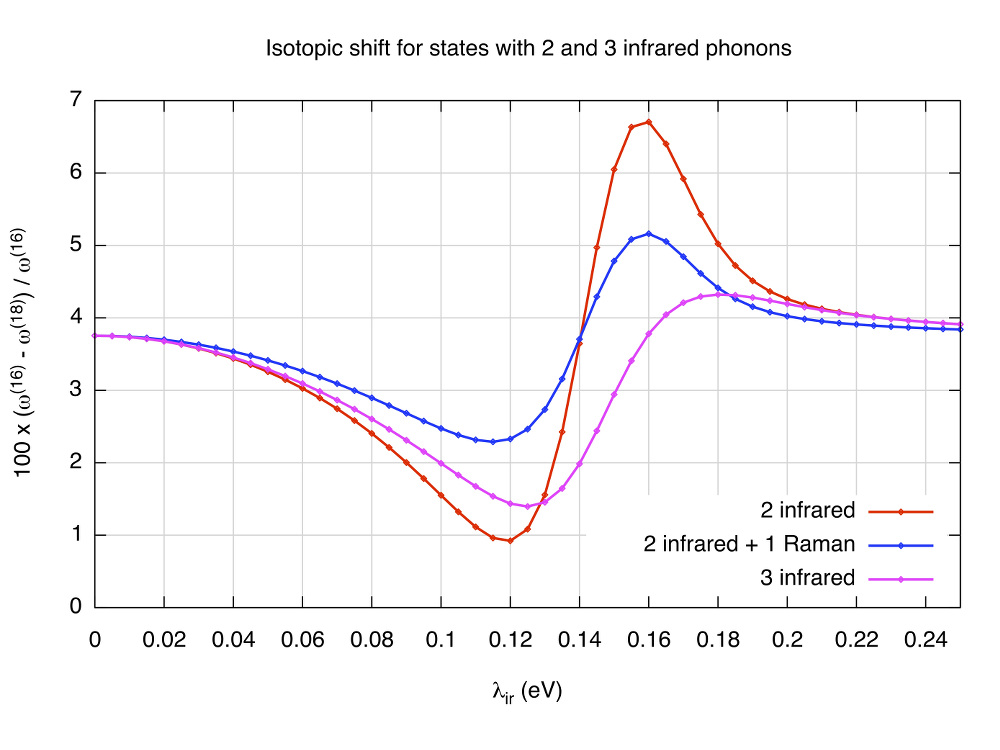
\includegraphics[width=0.8\textwidth]{images/isot-2_3ir.jpg}
\caption{Projection into phonon coordinates of the state with 3 infrared phonons.}
\label{fig:isot-2_3ir}
\end{figure}
